\subsection{Breadth-first search analysis}
\label{app:bfs-analysis}
\label{sec:exp-baselines}
\label{sec:results-baseline}

The saved BFS evaluation contains 725 attempts: 366/669 solved on easy samples
(54.7\%), 1/40 on medium, and 0/16 on hard. These attempts include repeated samples
and different budgets and are not paired with the recent ten-sample ablations.
BFS uses wall-clock, state-expansion, and depth limits, while model runs use turn
and call-timeout limits.
% Source: workspace/RESULTS/results.md.

A fold is specified by a line in current-plane coordinates together with a layer selection, and
both are drawn from small finite sets. Candidate lines are read off the crease pattern itself: the distinct lines through its mountain and valley edges,
carried forward through each distinct face transform into current coordinates, then deduplicated.
On a box-pleated pattern thousands of crease edges collapse to a few dozen lines. Layer selections
are not arbitrary subsets either, because a partial fold must be a contiguous run at one extremity
of the stack; the selections are the whole stack, the top $k$, and the bottom $k$, which is about
$2N$ for $N$ layers rather than $2^N$, with the over or under direction forced for partials. Each
surviving candidate is judged by the same function the \texttt{add\_fold} tool calls, so a listed
fold cannot be one the tool would then reject, and it is dropped if it fails any material check of
Section~\ref{sec:env-refusals} or would crease the sheet where the target pattern carries no
crease.

Across 73,750 enumerations recorded in the saved runs, this evaluates a mean of about 2,010
candidate actions per state and returns 3.51 of them, a ratio of approximately 570 between evaluated and returned candidates.
The baseline expands with the same enumerator the model is given, tests goals with the
same terminal comparator that decides \texttt{solved}, reads no reference sequence, and runs under
a per-sample wall-clock budget with caps on states expanded and depth.

% Included by sections/appendix-bfs.tex. Regenerate with
%   node workspace/figures/make_depth_wall_figure.mjs \
%     --data workspace/depth_wall/depth_wall.csv --enum workspace/enum_cost/enum_cost.json
% then copy workspace/figures/out/depth_wall.tex here and drop the standalone wrapper.
\begin{figure}[t]
\centering
% BFS depth wall, one curve per tier.
% Cost model: t(d) = b^d * c0 * g^d, with the per-node enumeration cost measured
% Generated by workspace/figures/make_depth_wall_figure.mjs
% Source: workspace/depth_wall/depth_wall.csv
% easy: b = 2.721, g = 1.441, c0 = 4.26e-3s (b*g = 3.92, 14 profiled states), reference depth 6.8, predicted 46 s (b fitted on 7 budget-exhausted runs over 3 samples)
% mid: b = 3.147, g = 1.472, c0 = 1.49e-2s (b*g = 4.63, 11 profiled states), reference depth 12.0, predicted 17 d (b fitted on 12 budget-exhausted runs over 3 samples)
% hard: b = 7.050, g = 1.758, c0 = 3.18e-1s (b*g = 12.39, 12 profiled states), reference depth 19.0, predicted 5.9e+12 y (b fitted on 8 budget-exhausted runs over 2 samples)
%
% Standalone: pdflatex depth_wall.tex
% In a paper: keep the tikzpicture, drop the documentclass wrapper.
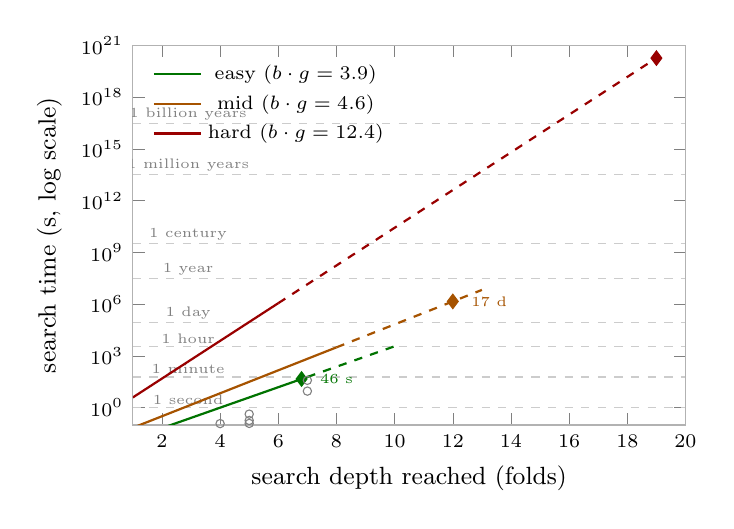
\begin{tikzpicture}
\begin{axis}[
  width=8.6cm, height=6.4cm,
  ymode=log,
  xlabel={search depth reached (folds)},
  ylabel={search time (s, log scale)},
  xmin=1, xmax=20, ymin=1e-1, ymax=1e21,
  xtick={2,4,6,8,10,12,14,16,18,20},
  ytick={1e0,1e3,1e6,1e9,1e12,1e15,1e18,1e21},
  tick label style={font=\scriptsize},
  label style={font=\small},
  legend style={font=\scriptsize, at={(0.02,0.98)}, anchor=north west, draw=none, fill=none},
  axis line style={gray!60},
]
\draw[gray!40, dashed, thin] (axis cs:1,1.0000e+0) -- (axis cs:20,1.0000e+0)
  node[pos=0.10, above, font=\tiny, gray, inner sep=1pt] {1 second};
\draw[gray!40, dashed, thin] (axis cs:1,6.0000e+1) -- (axis cs:20,6.0000e+1)
  node[pos=0.10, above, font=\tiny, gray, inner sep=1pt] {1 minute};
\draw[gray!40, dashed, thin] (axis cs:1,3.6000e+3) -- (axis cs:20,3.6000e+3)
  node[pos=0.10, above, font=\tiny, gray, inner sep=1pt] {1 hour};
\draw[gray!40, dashed, thin] (axis cs:1,8.6400e+4) -- (axis cs:20,8.6400e+4)
  node[pos=0.10, above, font=\tiny, gray, inner sep=1pt] {1 day};
\draw[gray!40, dashed, thin] (axis cs:1,3.1558e+7) -- (axis cs:20,3.1558e+7)
  node[pos=0.10, above, font=\tiny, gray, inner sep=1pt] {1 year};
\draw[gray!40, dashed, thin] (axis cs:1,3.1558e+9) -- (axis cs:20,3.1558e+9)
  node[pos=0.10, above, font=\tiny, gray, inner sep=1pt] {1 century};
\draw[gray!40, dashed, thin] (axis cs:1,3.1558e+13) -- (axis cs:20,3.1558e+13)
  node[pos=0.10, above, font=\tiny, gray, inner sep=1pt] {1 million years};
\draw[gray!40, dashed, thin] (axis cs:1,3.1558e+16) -- (axis cs:20,3.1558e+16)
  node[pos=0.10, above, font=\tiny, gray, inner sep=1pt] {1 billion years};
\addplot[thick, color=green!45!black, mark=none] coordinates {
  (1,1.66830e-2)
  (2,6.54005e-2)
  (3,2.56383e-1)
  (4,1.00507e+0)
  (5,3.94007e+0)
  (6,1.54458e+1)
  (7,6.05506e+1)
};
\addlegendentry{easy ($b\cdot g=3.9$)}
\addplot[thick, dashed, color=green!45!black, mark=none, forget plot] coordinates {
  (7,6.05506e+1)
  (8,2.37370e+2)
  (9,9.30537e+2)
  (10,3.64789e+3)
};
\addplot[thick, color=orange!65!black, mark=none] coordinates {
  (1,6.89243e-2)
  (2,3.19313e-1)
  (3,1.47932e+0)
  (4,6.85338e+0)
  (5,3.17504e+1)
  (6,1.47093e+2)
  (7,6.81456e+2)
  (8,3.15705e+3)
};
\addlegendentry{mid ($b\cdot g=4.6$)}
\addplot[thick, dashed, color=orange!65!black, mark=none, forget plot] coordinates {
  (8,3.15705e+3)
  (9,1.46260e+4)
  (10,6.77595e+4)
  (11,3.13917e+5)
  (12,1.45432e+6)
  (13,6.73756e+6)
};
\addplot[thick, color=red!60!black, mark=none] coordinates {
  (1,3.94464e+0)
  (2,4.88768e+1)
  (3,6.05619e+2)
  (4,7.50405e+3)
  (5,9.29805e+4)
  (6,1.15209e+6)
};
\addlegendentry{hard ($b\cdot g=12.4$)}
\addplot[thick, dashed, color=red!60!black, mark=none, forget plot] coordinates {
  (6,1.15209e+6)
  (7,1.42753e+7)
  (8,1.76881e+8)
  (9,2.19168e+9)
  (10,2.71564e+10)
  (11,3.36487e+11)
  (12,4.16932e+12)
  (13,5.16608e+13)
  (14,6.40114e+14)
  (15,7.93146e+15)
  (16,9.82765e+16)
  (17,1.21772e+18)
  (18,1.50884e+19)
  (19,1.86955e+20)
};
\addplot[only marks, mark=diamond*, mark size=2.6pt, color=green!45!black, forget plot]
  coordinates {(6.80,4.60741e+1)};
\node[font=\tiny, color=green!45!black, anchor=west] at (axis cs:7.10,4.60741e+1) {46 s};
\addplot[only marks, mark=diamond*, mark size=2.6pt, color=orange!65!black, forget plot]
  coordinates {(12.00,1.45432e+6)};
\node[font=\tiny, color=orange!65!black, anchor=west] at (axis cs:12.30,1.45432e+6) {17 d};
\addplot[only marks, mark=diamond*, mark size=2.6pt, color=red!60!black, forget plot]
  coordinates {(19.00,1.86955e+20)};

\addplot[only marks, mark=o, mark size=1.5pt, color=gray, forget plot] coordinates {
  (4,1.20000e-1)
  (5,4.25000e-1)
  (5,1.82000e-1)
  (5,1.23000e-1)
  (7,9.14900e+0)
  (7,3.87370e+1)
};
\end{axis}
\end{tikzpicture}
\caption{\textbf{Breadth-first search time against search depth, by difficulty group.}
The vertical axis is logarithmic, so a straight line is exponential growth and its slope is
$\log(b\cdot g)$. Curves are $t(d)=c_0(b\cdot g)^d$, the product of two exponentials: the
frontier grows as $b^d$ for a deduplicated branching factor $b$, measured as generated over
expanded during search, while the cost of expanding one node grows as $g^d$, because one
enumeration evaluates $4\times(\text{distinct crease lines})\times(\text{facets})$ candidates
and a fold of all layers at most doubles the facets. $g$ and $c_0$ are fitted by least squares
on per-depth enumeration timings. Each curve is solid only where that group was observed and
dashed beyond, and spans only the depths its own corpus reaches. Diamonds are each group's
mean reference depth; the hard group's sits at $10^{20}$ seconds, which is why the axis runs
that far. Circles are observed solves. $b$ is fitted from budget-exhausted runs: 7 over 3
samples for easy, 12 over 3 for medium, and 8 over 2 for hard, across 5 time budgets. The
hard extrapolation rests on two samples. Extrapolated values are model projections,
not measured solution times or lower bounds.}
\label{fig:depth-wall}
\end{figure}


The supplementary cost model approximates search time as the product of two exponential factors:
the frontier grows with the branching factor, and the cost of expanding one node grows with depth
as well, because one enumeration evaluates four candidates per crease line per facet and a fold of
all layers at most doubles the facets. Fitting both from the saved searches gives a per-fold
multiplier of 3.9 on the easy group, 4.6 on medium and 12.4 on hard
(Figure~\ref{fig:depth-wall}). These fitted curves extrapolate beyond the observed depths; they are not measured
solution times or lower bounds. The hard-group fit uses only two samples.
% EDITING NOTE: Validate the cost model and extrapolations before submission.


% Source: workspace/RESULTS/results.md, Deterministic search baseline.
% Static TeX bars; no additional plotting package or runtime required.
\begin{figure}[t]
\centering
\small
\begin{tabular}{llr}
Stratum (reference folds) & Median states expanded & Solved / attempts \\
\hline
Easy (4--10) & \rule{0.247cm}{8pt}\quad 65 & 366/669 \\
Medium (11--13) & \rule{4cm}{8pt}\quad 1,051.5 & 1/40 \\
Hard (14--19) & \rule{2.024cm}{8pt}\quad 532 & 0/16 \\
\end{tabular}
\caption{Observed BFS search effort in the saved aggregate. Bar lengths use a linear scale and
show median states expanded across attempts, including unsuccessful attempts. Budgets and repeated
samples are not standardized by this aggregate; 358 of 725 attempts terminated in timeout.
The lower hard-stratum median does not imply that hard instances require less search.
Reference depth is not minimum solution length.}
\label{fig:bfs-effort}
\end{figure}

